\documentclass{config/apuntes}

\title{Bioinformática Estructural}
\author{Sandra Mingo Ramírez}
\date{2024/25}
\acronym{STRBIO}

\usepackage[all]{nowidow}
\usepackage{listing}
\usepackage{color}
\usepackage{tabularx}
\usepackage{multirow}
\usepackage{makecell}
\usepackage{amsmath}
\usepackage{array}
\usepackage{soul}

\definecolor{dkgreen}{rgb}{0,0.6,0}
\definecolor{gray}{rgb}{0.5,0.5,0.5}
\definecolor{mauve}{rgb}{0.58,0,0.82}

\lstset{
  frame=tb,
  aboveskip=3mm,
  belowskip=3mm,
  showstringspaces=false,
  columns=flexible,
  basicstyle={\small\ttfamily},
  numbers=none,
  numberstyle=\tiny\color{gray},
  keywordstyle=\color{blue},
  commentstyle=\color{dkgreen},
  stringstyle=\color{mauve},
  breaklines=true,
  breakatwhitespace=true,
  tabsize=3
}

\usepackage{tocloft}

\advance\cftchapnumwidth 0.9em\relax
\advance\cftsecnumwidth 0.6em\relax
\advance\cftsubsecindent 0.5em\relax
\advance\cftsubsecnumwidth 0.5em\relax
\begin{document}

\begin{abstract}
La biología estructural permite el estudio de las estructuras de macromoléculas, el origen de esta estructura y su relación con la función biológica. La función específica está íntimamente ligada a la conformación tridimensional; la configuración estructural de las biomoléculas depende a su vez de su composición básica. Por ello, se busca obtener y comprender diferentes resultados de modelado de estructuras proteicas para resolver problemas biológicos. También es importante comprender las bases teóricas, tanto conceptuales como algorítmicas, de la predicción y análisis de estructura de macromoléculas, e interpretar los resultados de estos programas.

Apuntes adaptados a partir de los proporcionados por Modesto Redrejo en \href{https://strbio.github.io/}{https://strbio.github.io/}
\end{abstract}

\pagestyle{plain}

\maketitle

\tableofcontents

%Tema 1: Aplicaciones y métodos de bioinformática estructural en biología y biomedicina
%Tema 2: Aplicaciones para visualización de estructuras 3D de moléculas biológicas
%Tema 3: Métodos alternativos para la predicción de estructuras secundarias y terciarias de proteínas
%Tema 4: Acoplamiento (docking) computacional de proteínas y fármacos
%Examen 40% 
%Prácticas 60%
	%5% play with secondary structures and protein DDBB
	%15% working with structures
	%30% casp-like exercise
	%5% randomized peer-assessment -> opcional, es un 5% adicional en la asignatura
	%10% docking
	%Electronic Lab Notebook: esto es el objetivo, esto es lo que hemos hecho, esto es lo que hemos conseguido

%29/01 - Modesto
\part{Introducción y modelado de proteínas}
\chapter{Aplicaciones y métodos de bioinformática estructural en biología y biomedicina}
\section{Metas en la bioinformática estructural}
La bioinformática estructural (SB por sus siglas en inglés) es una disciplina amplia que abarca recursos de datos, algoritmos y herramientas para investigar, analizar, predecir e interpretar estructuras biomacromoleculares. En este curso, nos centraremos específicamente en la bioinformática estructural de proteínas, incluyendo la visualización y el análisis de la estructura de biomacromoléculas, así como la predicción de estructuras y complejos de proteínas. La premisa de la SB es que la información estructural de alta resolución sobre los sistemas biológicos permite un razonamiento preciso sobre sus funciones y los efectos de las modificaciones y perturbaciones.

Los objetivos de SB requieren al menos cuatro líneas de investigación diferentes:
\begin{itemize}
\item \textbf{Visualización}: Tratar con una o muchas estructuras complejas e integrar varias fuentes de información como secuencias, datos estructurales, campos electrostáticos, localizaciones de sitios funcionales y áreas de variabilidad.
\item \textbf{Clasificación}: Agrupación jerárquica de estructuras similares para identificar orígenes comunes y vías de diversificación. Al igual que en otros campos de la biología, la clasificación es tediosa pero necesaria para comprender el espacio estructural.
\item La \textbf{predicción} de estructuras sigue siendo un área de gran interés y un campo de investigación en sí mismo. Como veremos a continuación, el número de secuencias diferentes es mucho mayor que la disponibilidad de estructuras, lo que hace de la predicción una herramienta esencial y útil.
\item \textbf{Simulación}: Las estructuras obtenidas experimentalmente son ante todo modelos estructurales estáticos. Sin embargo, las propiedades de estas moléculas son a menudo el resultado de sus movimientos dinámicos. La definición de las funciones energéticas que rigen el plegamiento de las proteínas y su posterior dinámica estable pueden analizarse mediante simulaciones de dinámica molecular, aunque las capacidades de cálculo pueden ser limitantes para alcanzar escalas de tiempo biológicamente relevantes.
\end{itemize}

Impulsado por enormes cantidades de datos e importantes avances técnicos, este campo ha experimentado una transformación sustancial en los últimos veinte años. La mejora de las capacidades experimentales para analizar la estructura de las proteínas y otras moléculas y estructuras biológicas y el avance de la predicción de estructuras asistida por Inteligencia Artificial (IA) han aumentado sustancialmente la capacidad de los investigadores de las ciencias de la vida para abordar diversas cuestiones relativas a la diversidad, evolución y función de las proteínas. Esta transformación se ha potenciado en los últimos 5 años, y sus implicaciones para la biología, la biotecnología y la biomedicina siguen siendo en gran medida impredecibles.

\section{Introducción a las estructuras proteicas}
Las proteínas son componentes esenciales de la vida, que intervienen en diversas funciones vitales como elementos estructurales, elementos de andamiaje o enzimas activas que catalizan reacciones metabólicas. Las proteínas están compuestas por polímeros de aminoácidos, y la secuencia de aminoácidos de una proteína concreta se denomina \textbf{estructura primaria} de la proteína. Las cadenas de aminoácidos pueden plegarse espontáneamente en estructuras tridimensionales, estabilizadas principalmente por enlaces de hidrógeno entre aminoácidos. La secuencia de aminoácidos determina las diferentes capas de la estructura tridimensional. En la naturaleza existen L-aminoácidos, pero no D-aminoácidos. Cada uno de los 20 aminoácidos naturales tiene propiedades fisicoquímicas específicas que influyen en su conformación preferida. Por lo tanto, el nivel inicial de plegamiento se conoce como \textbf{estructura secundaria}, que forma patrones comunes como se verá más adelante. Estos segmentos de patrones de estructura secundaria son capaces de plegarse en formas tridimensionales debido a las interacciones entre las cadenas laterales de los aminoácidos, lo que se conoce como \textbf{estructura terciaria} de la proteína. Además, dos o más cadenas peptídicas individuales pueden agregarse para formar proteínas multisubunidad, lo que se conoce como \textbf{estructura cuaternaria}.

\begin{figure}[h]
\centering
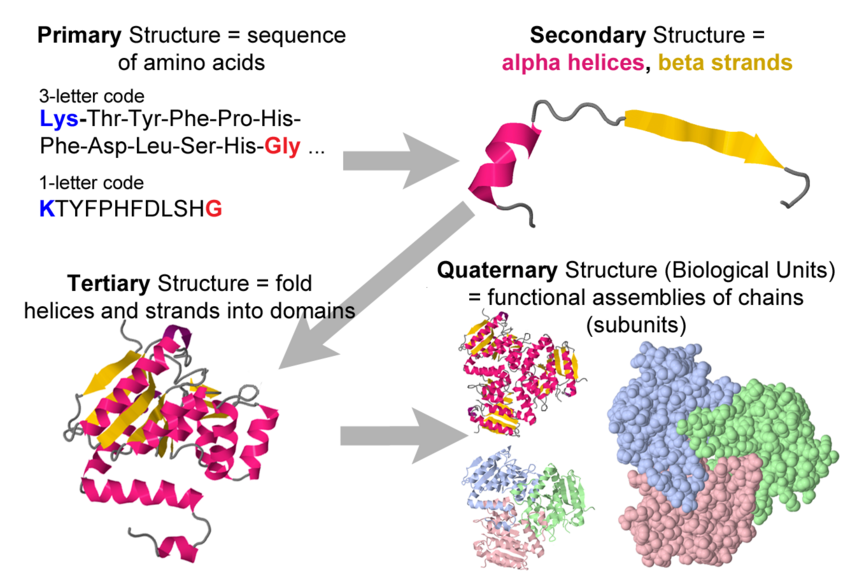
\includegraphics[width = 0.6\textwidth]{figs/850px-Protein-structure-4-levels-III-flat.png}
\caption{Los distintos niveles de la estructura proteica.}
\end{figure}

Es importante señalar que el enlace peptídico en sí no permite la rotación, ya que posee características parciales de doble enlace. Por lo tanto, la rotación está restringida a los enlaces entre el C$\alpha$ y el grupo C = O (el ángulo phi ($\phi$)) y el C$\alpha$ y el grupo NH (el ángulo psi ($\psi$)). Así pues, la cadena principal del polipéptido consiste en una secuencia repetida de dos enlaces giratorios seguidos de un enlace no giratorio (péptido). Sin embargo, no todos los 360º de los ángulos $\phi$ y $\psi$ son factibles debido a posibles \textbf{choques estéricos} entre cadenas laterales vecinas. Para determinados ángulos y combinaciones de aminoácidos, las restricciones espaciales impiden que los átomos ocupen la misma ubicación física, lo que explica en parte las distintas propensiones de ciertos aminoácidos a adoptar diferentes tipos de estructuras secundarias. 

\begin{figure}[h]
\centering
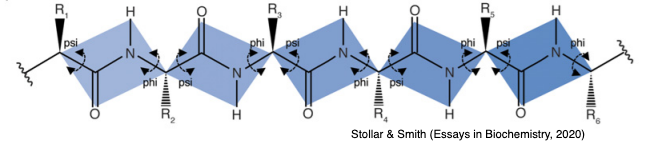
\includegraphics[width = 0.8\textwidth]{figs/peptide_bond.png}
\caption{Esquema de una cadena polipeptídica genérica. Las cadenas laterales de los residuos se denotan como R. Los rectángulos coloreados indican conjuntos de seis átomos que son coplanares debido al carácter de doble enlace del enlace peptídico. Las flechas indican los enlaces que son libres de rotar con el ángulo de rotación sobre el N-C$\alpha$ conocido como phi ($|phi$) y sobre el C$\alpha$-C conocido como psi ($\psi$). Obsérvese que sólo se etiquetan los enlaces del esqueleto peptídico y que, en la mayoría de los casos, el enlace del grupo R es libre de rotar.}
\end{figure}

Además, las cadenas laterales de los aminoácidos poseen sus propios ángulos de torsión, conocidos como $\chi1$, $\chi2$, $\chi3$, etc (figura \ref{fig:chi}). Estos ángulos de torsión influyen significativamente en las estructuras secundarias y, sobre todo, terciarias de las proteínas. Las distintas combinaciones de torsiones de las cadenas laterales definidas por los ángulos $\chi$ se denominan \textbf{rotámeros}.

\begin{figure}[h]
\centering
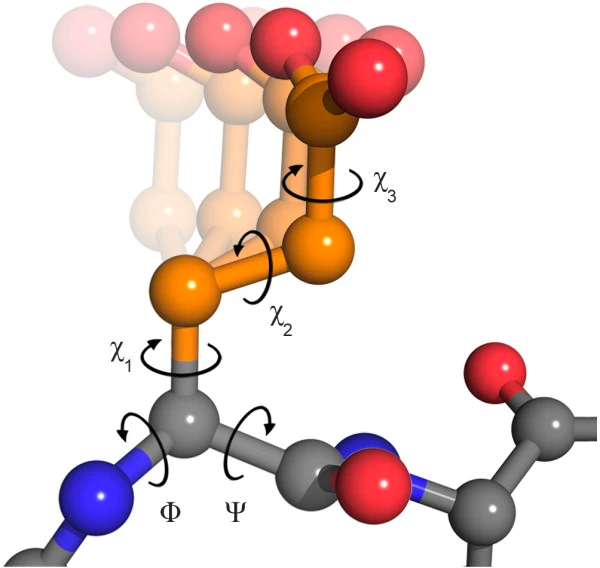
\includegraphics[width = 0.3\textwidth]{figs/paste-6EE800AE.png}
\caption{Ángulos diedros en el glutamato: Los ángulos diedros son los principales grados de libertad de la columna vertebral (ángulos $\phi$ y $\psi$) y la cadena lateral (ángulos $\chi$) de un aminoácido. El número de ángulos $\chi$ varía entre cero y cuatro para los 20 aminoácidos estándar. La figura muestra una representación esférica del glutamato, que tiene tres $\chi$ ángulos.}
\label{fig:chi}
\end{figure}

Dentro de estas limitaciones, las dos conformaciones locales primarias que evitan el impedimento estérico y maximizan el enlace de hidrógeno entre la columna vertebral y el backbone son las estructuras secundarias $\alpha$-hélice y $\beta$-hoja. Linus Pauling propuso inicialmente la hélice $\alpha$ como zurda en 1951, pero la estructura cristalina de la mioglobina en 1958 reveló que la forma diestra es más común. En las hélices diestras típicas, el grupo NH de la espina dorsal se une mediante enlaces de hidrógeno al grupo C=O de la espina dorsal del aminoácido situado cuatro residuos antes en la secuencia de la proteína. Esta forma de espiral regular tiene los grupos R apuntando hacia fuera, lejos de la espina dorsal peptídica, y requiere unos 3,6 residuos para completar una vuelta completa de la hélice (figura \ref{fig:alfa}).

\begin{figure}[h]
\centering
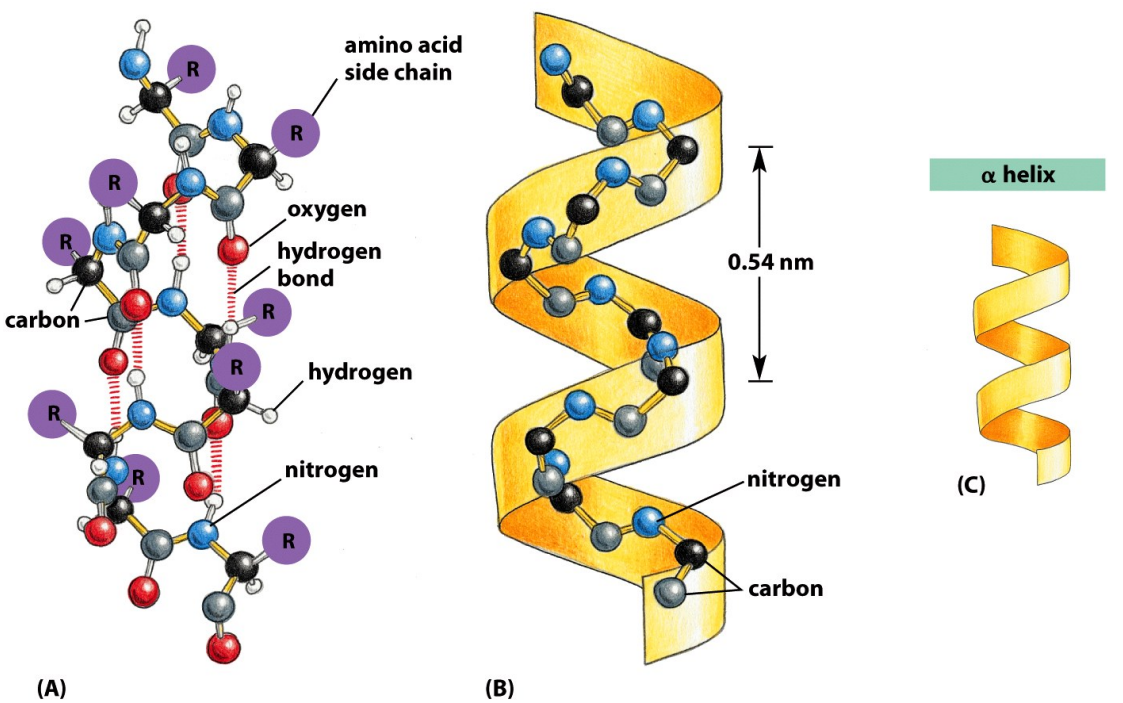
\includegraphics[width = 0.6\textwidth]{figs/alpha.png}
\caption{Hélice alfa.}
\label{fig:alfa}
\end{figure}

Las diferentes secuencias de aminoácidos tienen distintas tendencias a formar estructuras $\alpha$-helicoidales. La metionina, la alanina, la leucina, el glutamato y la lisina tienen propensiones especialmente altas a formar hélices, mientras que la prolina y la glicina tienen propensiones pobres a formar hélices. La prolina a menudo rompe o retuerce una hélice porque carece de un hidrógeno amida para formar enlaces de hidrógeno y su voluminosa cadena lateral interfiere con el esqueleto del giro precedente. La glicina, con sólo un hidrógeno como grupo R, es demasiado flexible y costosa desde el punto de vista entrópico para mantener la estructura $\alpha$-helicoidal, lo que la convierte en una rompedora de hélices $\alpha$.

\begin{figure}[h]
\centering
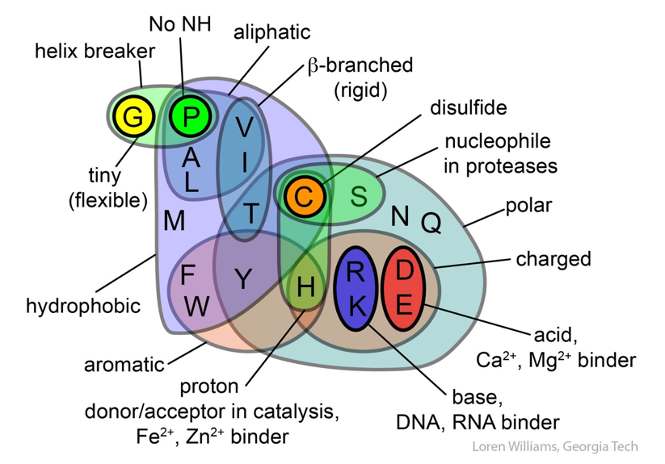
\includegraphics[width = 0.5\textwidth]{figs/aa.png}
\caption{Aminoácidos clasificados según su tipo.}
\end{figure}

Las láminas $\beta$ (figura \ref{fig:beta}) están formadas por dos o más cadenas polipeptídicas extendidas denominadas hebras $\beta$ que discurren una junto a otra en disposición paralela o antiparalela. En una lámina $\beta$, los residuos se disponen en zigzag y los enlaces peptídicos adyacentes apuntan en direcciones opuestas. El grupo NH y el grupo C=O de cada aminoácido forman enlaces de hidrógeno con el grupo C=O y el grupo NH, respectivamente, de las cadenas adyacentes. Las cadenas pueden ir en direcciones opuestas (lámina $\beta$ antiparalela) o en la misma dirección (lámina $\beta$ paralela). Las cadenas laterales de cada residuo se alternan en direcciones opuestas, dando a las láminas $\beta$ caras hidrofílicas e hidrofóbicas, formando a menudo un patrón de alternancia de residuos hidrofílicos e hidrofóbicos en la estructura primaria.

\begin{figure}[h]
\centering
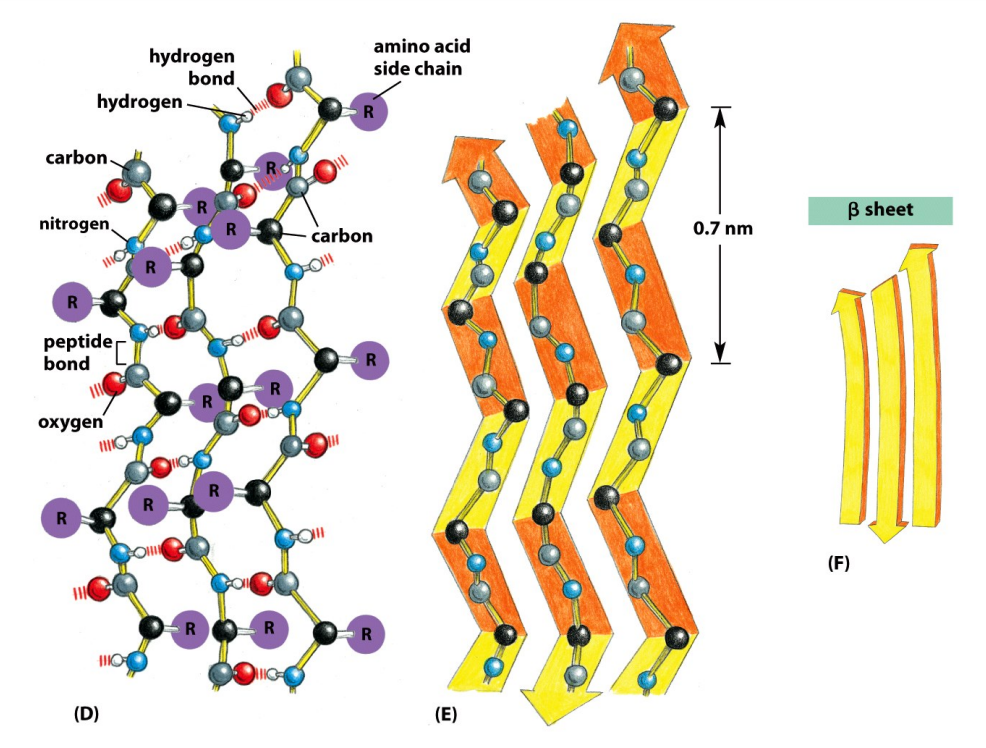
\includegraphics[width = 0.6\textwidth]{figs/beta.png}
\caption{Descripción detallada de una lámina beta formada por tres hebras beta.}
\label{fig:beta}
\end{figure}

Los residuos aromáticos grandes (tirosina, fenilalanina, triptófano) y los aminoácidos $\beta$-ramificados (treonina, valina, isoleucina) suelen encontrarse en las hebras $\beta$. Como en el caso de las hélices $\alpha$, las hebras $\beta$ suelen estar terminadas por glicinas, que son especialmente comunes en los giros $\beta$ (el conector más común entre hebras), como aminoácidos con ángulos $\phi$ positivos.

Las estructuras secundarias, terciarias y cuaternarias de las proteínas se mantienen gracias a las interacciones entre aminoácidos (figura \ref{fig:interactions}). Estas interacciones suelen clasificarse en cuatro tipos, que pueden ser tanto intra- como intermoleculares:
\begin{enumerate}
\item \textbf{Enlace iónico}: Los enlaces iónicos surgen de las atracciones electrostáticas entre cadenas laterales de aminoácidos cargadas positiva y negativamente. Por ejemplo, la atracción entre un ion carboxilato del ácido aspártico y un ion amonio de la lisina ayuda a estabilizar una región plegada específica de una proteína.
\item \textbf{Enlace de hidrógeno}: Los enlaces de hidrógeno se forman entre un átomo de oxígeno o nitrógeno altamente electronegativo y un átomo de hidrógeno unido a otro átomo de oxígeno o nitrógeno, como los de las cadenas laterales de aminoácidos polares. Los enlaces de hidrógeno son cruciales para las interacciones intra e intermoleculares en las proteínas, como en las hélices alfa.
\item \textbf{Enlaces disulfuro}. Cuando dos aminoácidos cisteína se acercan durante el plegamiento de la proteína en condiciones redox adecuadas, la oxidación puede unir sus átomos de azufre, formando un enlace disulfuro. A diferencia de los enlaces iónicos o de hidrógeno, se trata de enlaces covalentes, por lo que son un ejemplo clásico de reacción espontánea, que se produce como modificación postraduccional. Aunque son sensibles a los agentes reductores, estabilizan en gran medida la estructura terciaria y son vitales para la estructura cuaternaria de muchas proteínas, como los anticuerpos.
\item \textbf{Interacciones hidrofóbicas}. Las fuerzas de dispersión surgen cuando un átomo normalmente no polar se convierte momentáneamente en polar debido a una distribución desigual de electrones, dando lugar a un dipolo instantáneo que induce un desplazamiento de electrones en un átomo no polar vecino. Las fuerzas de dispersión son débiles, pero pueden ser importantes cuando otros tipos de interacciones no existen o son mínimas. El término interacción hidrofóbica suele utilizarse erróneamente como sinónimo de fuerzas de dispersión. Las interacciones hidrofóbicas surgen porque las moléculas de agua establecen enlaces de hidrógeno con otras moléculas de agua (o grupos de proteínas capaces de establecer enlaces de hidrógeno). Como los grupos no polares no pueden formar enlaces de hidrógeno, la proteína se pliega de tal forma que estos grupos quedan enterrados en la parte interior de la estructura proteica, minimizando su contacto con el agua.
\end{enumerate}

\begin{figure}[h]
\centering
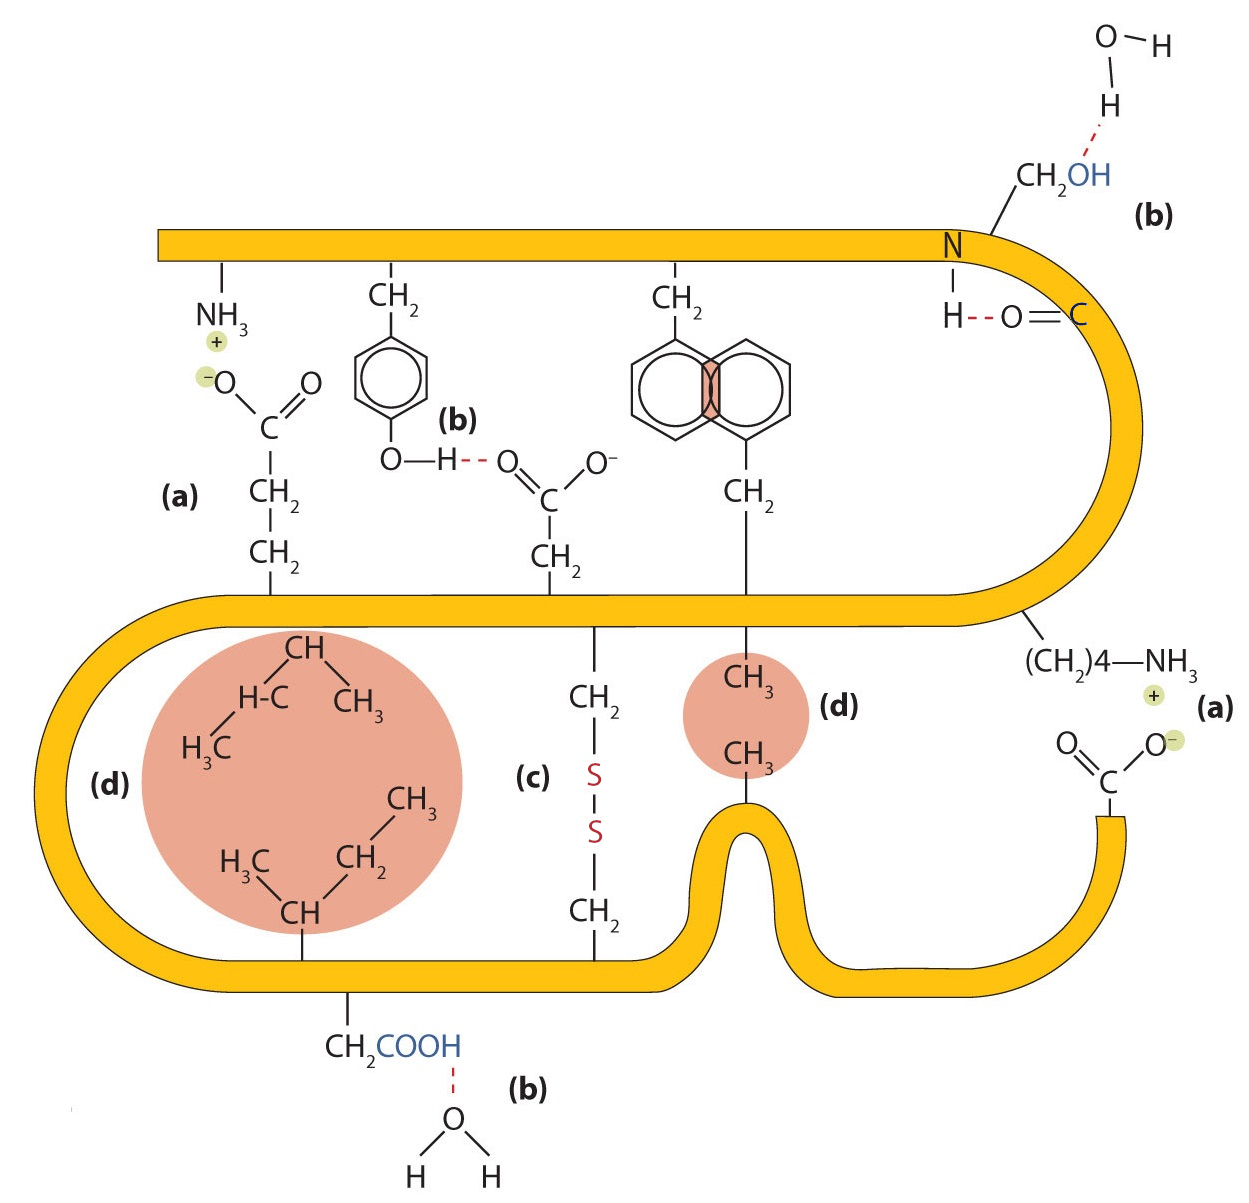
\includegraphics[width = 0.6\textwidth]{figs/interactions-01.png}
\caption{Cuatro interacciones estabilizan la estructura terciaria de una proteína: (a) enlace iónico, (b) enlace de hidrógeno, (c) enlaces disulfuro y (d) fuerzas de dispersión.}
\label{fig:interactions}
\end{figure}

Otras interacciones intramoleculares menos frecuentes podrían ser relevantes en algunas proteínas, como los llamados enlaces isopéptidos, formados entre dos grupos proteicos, al menos uno de los cuales no es un grupo $\alpha$-amino o $\alpha$-carboxi. Algunos ejemplos son la ubiquitilación, la sumoilación, la transglutaminación, el anclaje de proteínas a la superficie celular mediado por sortasas y la formación de pilus. Todos estos procesos comparten varias características (figura \ref{fig:iso}):
\begin{itemize}
\item Todos implican la reacción de un grupo $\epsilon$-amino de la lisina de una proteína con el grupo $\alpha$-carboxi principal de otra proteína, excepto en el caso de la transglutaminación, en la que la lisina se dirige a un grupo carboxiamida de la cadena lateral de la glutamina.
\item Todos los procesos están mediados por enzimas e implican un intermediario tioéster transitorio formado por la cisteína del sitio activo. Este intermediario se resuelve mediante un ataque nucleofílico por el grupo $\epsilon$-amino de la lisina, que completa la formación del enlace.
\end{itemize}

\begin{figure}[h]
\centering
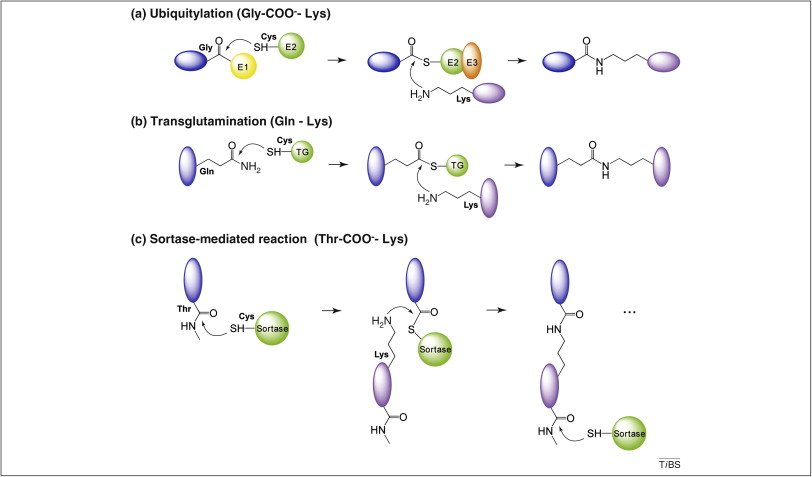
\includegraphics[width = 0.8\textwidth]{figs/iso.jpg}
\caption{Formación de enlaces isopeptídicos intermoleculares mediada por enzimas. Se muestran ejemplos de tres procesos biológicos diferentes: ubiquitilación, transglutaminación y ensamblaje de pilus mediado por sortasa en bacterias Gram positivas. Las proteínas unidas por enlaces isopeptídicos están coloreadas en azul y morado y las enzimas formadoras de enlaces isopeptídicos en verde.}
\label{fig:iso}
\end{figure}

A diferencia de estos procesos dependientes de enzimas, los enlaces isopeptídicos entrecruzados (intrachain isopeptide bonds) se forman autocatalíticamente en la pilina principal Spy0128 de \textit{S. pyogenes} y en otras proteínas de la superficie de células Gram+, así como en la cápside del fago HK97. En este caso, la reacción de formación del enlace es una reacción inducida por la proximidad que se produce cuando los aminoácidos participantes se sitúan juntos en un entorno hidrofóbico, ya sea a través del plegamiento de la proteína concurrente con la formación del enlace peptídico en el ribosoma o por la reorganización de la cápside (en HK97).

En cuanto a la ingeniería proteica, es posible crear aminoácidos no naturales reactivos. Esto se ha utilizado para aumentar la termoestabilidad de proteínas como anticuerpos, crear recombinantes y unir covalentemente proteínas a superficies o nanopartículas.

\subsection{Gráfico de Ramachandran}
Muchas combinaciones de ángulos $\phi$ y $\psi$ están prohibidas debido al principio de exclusión estérica, que dicta que dos átomos no pueden ocupar el mismo espacio simultáneamente. Este concepto fue demostrado inicialmente por Gopalasamudram Ramachandran, que desarrolló un gráfico para visualizar los valores de ángulo permitidos, conocido como gráfico de Ramachandran. Este gráfico puede mostrar los ángulos de un aminoácido específico, de todos los aminoácidos de una proteína o incluso de muchas proteínas. El análisis de los ángulos $\phi$ y $\psi$ en proteínas conocidas revela que aproximadamente tres cuartas partes de todas las combinaciones posibles de $\phi$, $\psi$ no están permitidas (figura \ref{fig:ramachandran}) y se corresponden con motivos comunes de estructura secundaria (figura \ref{fig:ramachandran2}).

\begin{figure}[h]
\centering
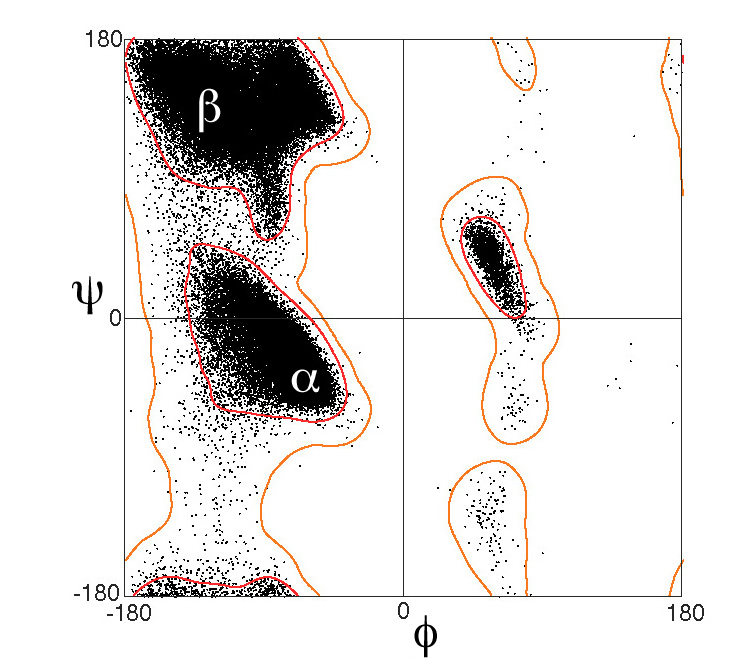
\includegraphics[width = 0.6\textwidth]{figs/Ramachandran_plot_general_100K.jpg}
\caption{Diagrama general de Ramachandran. La densidad de puntos refleja la probabilidad de cada combinación de ángulos, definiendo las regiones central (línea roja) y de tolerancia (naranja).}
\label{fig:ramachandran}
\end{figure}

\begin{figure}[h]
\centering
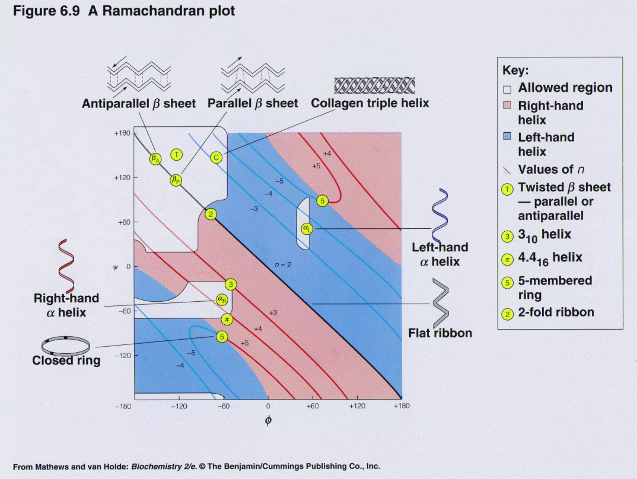
\includegraphics[width = 0.6\textwidth]{figs/rama2.png}
\caption{Definición de alternativas de estructura secundaria por su combinación de ángulos phi, psi.}
\label{fig:ramachandran2}
\end{figure}

Los residuos funcionalmente relevantes son más propensos que otros a tener ángulos de torsión que se sitúan en las regiones permitidas pero desfavorecidas de un diagrama de Ramachandran. La geometría específica de estos residuos relevantes desde el punto de vista funcional, aunque desfavorable desde el punto de vista energético, puede ser importante para la función de la proteína, ya sea catalítica o de otro tipo. Tales conformaciones deben ser estabilizadas por la proteína mediante enlaces H, empaquetamiento estérico u otros medios, y rara vez se dan en residuos muy expuestos a disolventes.

Suele haber espacios designados para las hélices $\alpha$ y las láminas $\beta$, pero también puede haber outliers que muestren aminoácidos concretos.

\subsection{Pliegues (folds), dominios y motivos de proteínas}
La estructura terciaria tridimensional global de una proteína se conoce comúnmente como su \textbf{pliegue}, definiendo así la forma y orientación global ignorando los loops. Dentro del pliegue proteico global, podemos reconocer distintos dominios y motivos. Los \textbf{dominios} son secciones compactas de la proteína que representan regiones estructural y (normalmente) funcionalmente independientes. Eso significa que un dominio mantiene sus características principales, aunque se separe de la proteína global. Por otro lado, los \textbf{motivos} son pequeñas subestructuras que no son necesariamente independientes y que constan sólo de unos pocos tramos de estructura secundaria. De hecho, los motivos también pueden denominarse superestructuras secundarias y son frecuentes en la secuencia. En resumen, un dominio corresponde a un fold, y una cadena peptídica puede tener uno o varios dominios.

La diversidad de pliegues, dominios y motivos proteicos, así como su combinación, puede utilizarse para clasificar jerárquicamente las estructuras proteicas, como en muchos otros campos de la biología. La primera clasificación se propuso en los años 70 y consistía en cuatro grupos de pliegues, como se muestra en la siguiente figura. Todas las proteínas $\alpha$ se basan casi por completo en una estructura $\alpha$-hélice, y todas las estructuras $\beta$ se basan en $\beta$-láminas. La estructura $\alpha$/$\beta$ se basa en una mezcla de $\alpha$-hélices y $\beta$-láminas, a menudo organizadas como $\beta$-hebras paralelas conectadas por $\alpha$-hélices. Por otro lado, las estructuras $\alpha$+$\beta$ consisten en motivos discretos de $\alpha$-hélice y $\beta$-lámina que no están entrelazados (como ocurre en las proteínas $\alpha$/$\beta$). Por último, las proteínas pequeñas abarcan polipéptidos con estructuras secundarias nulas o escasas.

\begin{figure}[h]
\centering
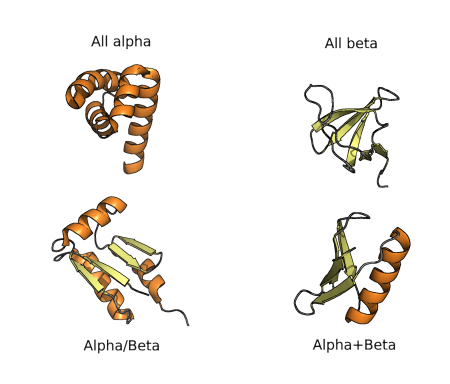
\includegraphics[width = 0.6\textwidth]{figs/clasif.png}
\caption{Las cuatro clases de proteínas estructurales de la clasificación de Chlothia y Levitt.}
\label{fig:alphabeta}
\end{figure}
%31/01 - Modesto
\chapter{Bases de datos de proteínas}
\section{Comparación de estructura y alineamiento}
Para comprender la diversidad y función de las proteínas, es importante comparar sus secuencias y estructuras. Esto ayuda a encontrar patrones comunes y a comprender su diversidad e historia evolutiva. Midiendo y analizando estas similitudes, los científicos pueden clasificar las proteínas y determinar sus relaciones en términos de función y evolución. Este proceso también es crucial en el modelado de proteínas, ya que ayuda a identificar, evaluar y elegir modelos intermedios.

Es esencial aclarar la distinción entre alineamiento y superposición, ya que estos términos se confunden con frecuencia en la literatura. Un \textbf{alineamiento estructural} pretende identificar similitudes y diferencias entre dos estructuras, mientras que la \textbf{superposición de estructuras} muestra las estructuras basándose en criterios específicos, normalmente derivados de un alineamiento estructural previo. Por consiguiente, la superposición trata de minimizar la distancia entre estructuras identificando una transformación que consiga la menor desviación cuadrática media (RMSD) o las máximas equivalencias dentro de un límite RMSD.

La RMSD puede calcularse para cualquier par de moléculas. En el contexto de las proteínas, solemos referirnos a la RMSD de los alfa-carbones. Una alineación superior facilitará una mejor superposición. Por lo tanto, aunque la alineación y la superposición son procesos distintos, la RMSD puede servir como indicador de ambos; cuanto menor sea la RMSD, mejor será la alineación/superposición. Es importante señalar que la RMSD es una medida de distancia real, no una puntuación. Eso implica que sólo podemos obtener la RMSD para los residuos alineados, no para toda la secuencia de cualquiera de las dos proteínas. Por lo tanto, una RMSD de 1 $\AA$ puede indicar una distancia cercana pero, si implica a muy pocos aminoácidos, no sugiere necesariamente una buena similitud. Tanto el valor RMSD como el número de residuos alineados deben tenerse en cuenta para un análisis preciso.

\begin{figure}[h]
\centering
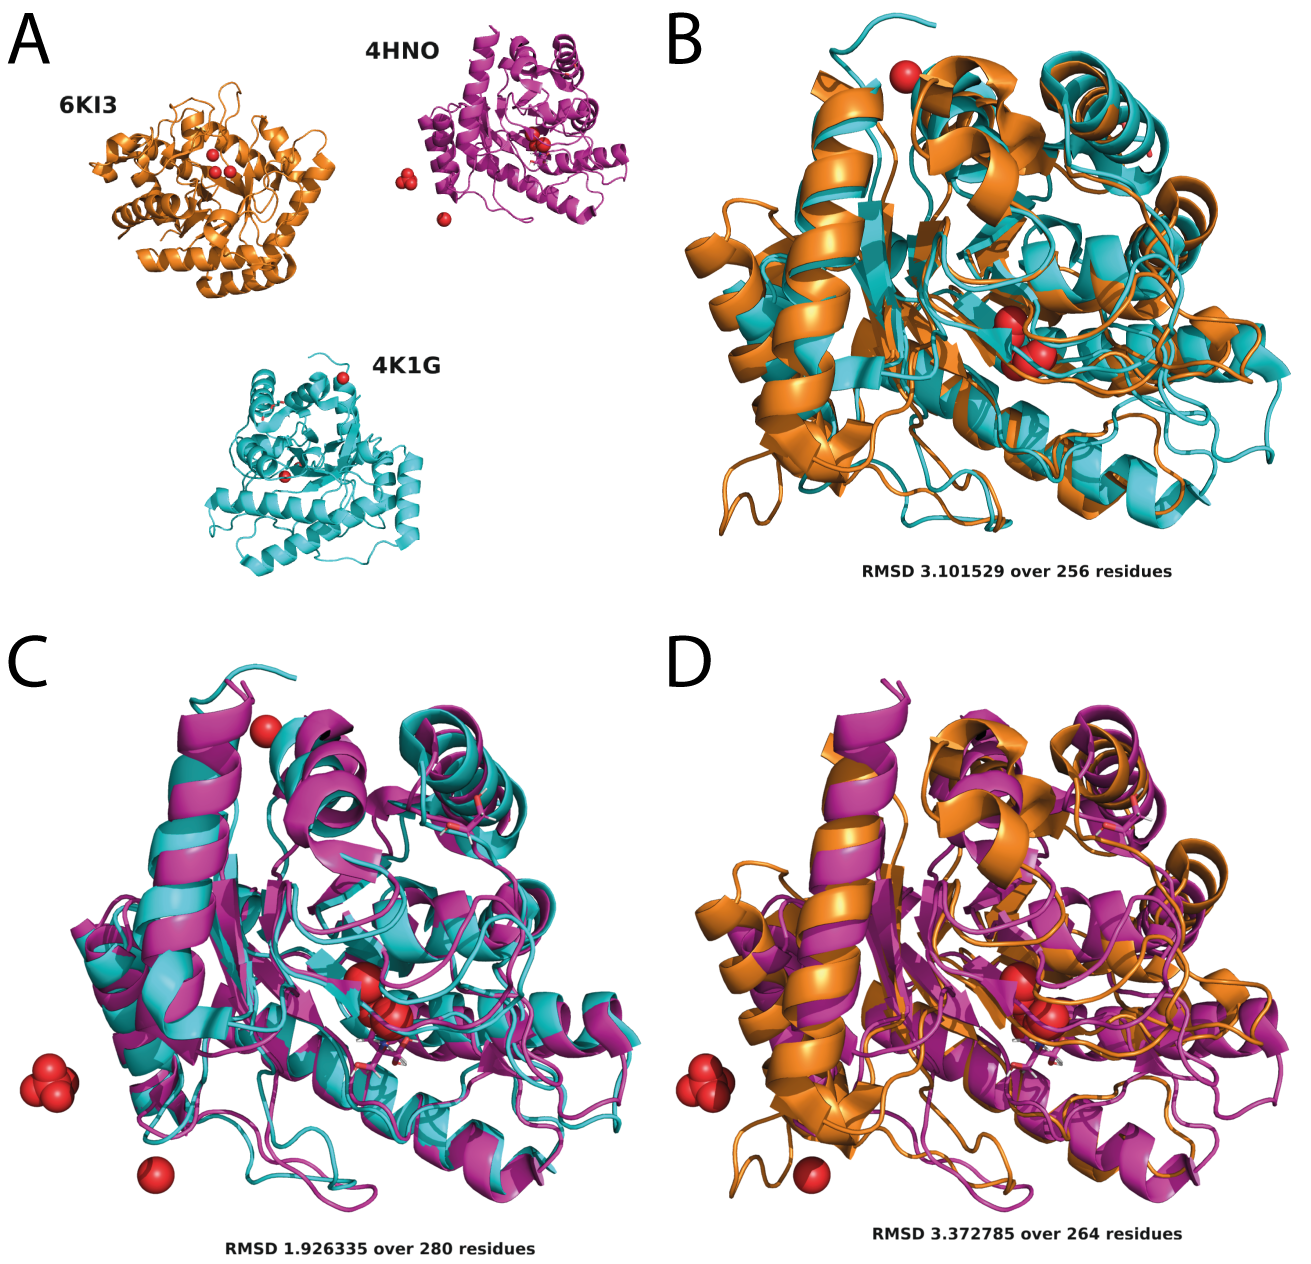
\includegraphics[width = 0.6\textwidth]{figs/rmsd.png}
\end{figure}

Global Distance Test se utiliza en CASP al ser menos sensible a outliers y permite comparar estructuras de secuencias idénticas. Se normaliza el número de residuos que caigan bajo un límite.

\section{Principales bases de datos de proteínas}
La clasificación de secuencias proteicas nos ayuda a comprender la diversidad de las distintas proteínas mediante el examen de sus secuencias, lo que se conoce como el \textbf{espacio de secuencias proteicas} (el concepto matemático de espacio). Por otro lado, la clasificación de las estructuras proteicas consiste en agrupar las proteínas en función de sus relaciones estructurales. Algunas clasificaciones tienen en cuenta la vecindad estructural (continuo estructural), mientras que otras utilizan el concepto de evolución de las proteínas como principal factor de diversificación, lo que da lugar a un \textbf{espacio de estructuras proteicas} discreto en lugar de continuo.

Esta sección no pretende ofrecer una revisión exhaustiva de todas las bases de datos de proteínas. En consecuencia, no cubriremos en detalle la base de datos de proteínas del NCBI, que se utiliza ampliamente para diversos fines y probablemente se mencione en otros cursos. La Base de Datos de Proteínas del NCBI sirve principalmente como repositorio principal de secuencias, con un énfasis mínimo en el análisis de la diversidad y clasificación de proteínas. Esta sección destacará las principales diferencias y aplicaciones de Pfam, Uniprot, Prosite, PDB, SCOP y CATH. 

\begin{figure}[h]
\centering
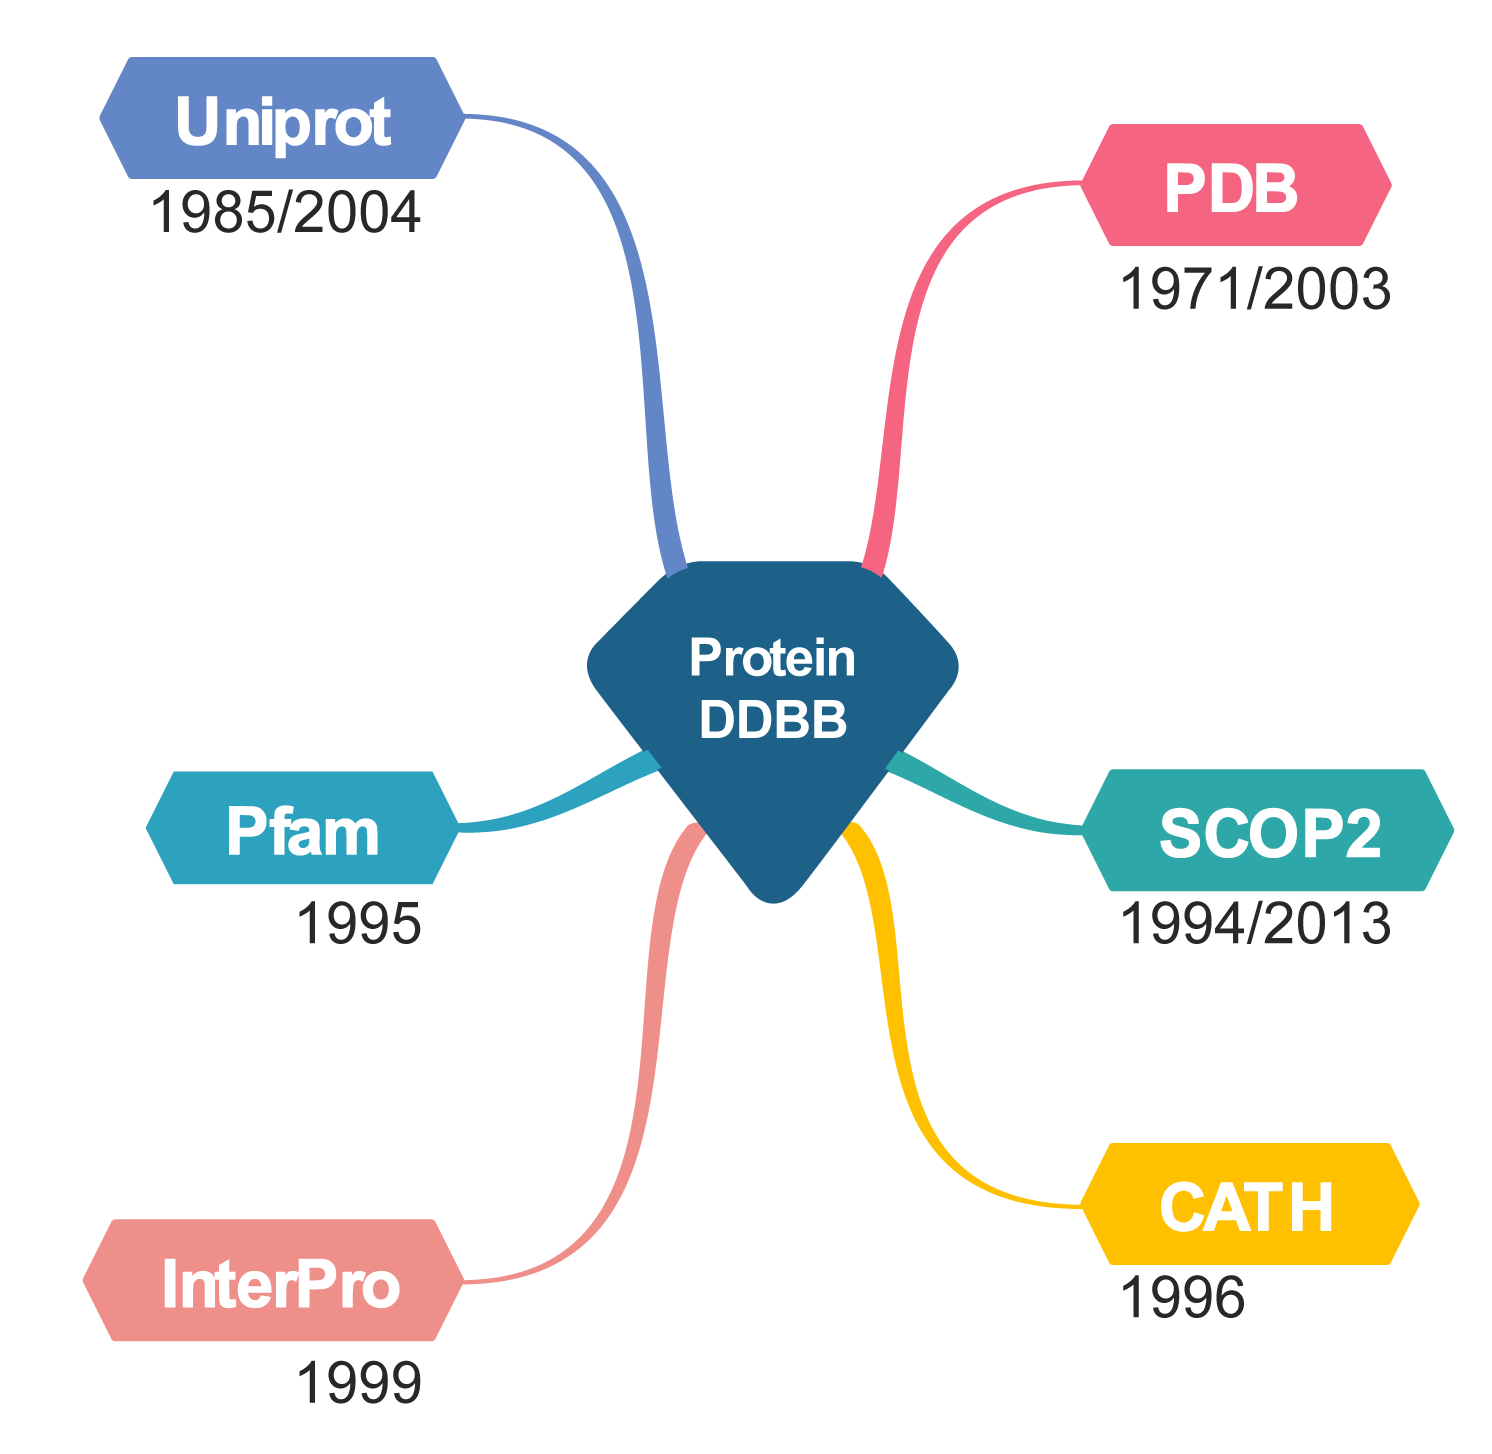
\includegraphics[width = 0.4\textwidth]{figs/ddbb.png}
\end{figure}

En bioinformática, las bases de datos suelen clasificarse en primarias o secundarias. Las \textbf{bases de datos primarias} contienen datos obtenidos experimentalmente, como secuencias de nucleótidos, secuencias de proteínas o estructuras macromoleculares. Es importante señalar que, una vez asignado el número de acceso a una base de datos, los datos de las bases de datos primarias permanecen inalterados y forman parte del registro científico. En cambio, las \textbf{bases de datos secundarias} incluyen datos derivados del análisis de datos primarios. Estas bases de datos suelen utilizar información procedente de numerosas fuentes, incluidas otras bases de datos y la literatura científica. Suelen ser muy complejas e implican una compleja combinación de algoritmos informáticos y/o análisis e interpretación manuales para generar nuevos conocimientos a partir del registro público de la ciencia.

Aunque la distinción entre bases de datos primarias y secundarias se ha vuelto menos clara en los últimos tiempos debido a la integración de datos procedentes de diversas fuentes, aún pueden distinguirse algunas diferencias. Las principales bases de datos primarias para secuencias de proteínas son NCBI Protein y RCSB-PDB para estructuras proteicas. UniProt también alberga una base de datos primaria de secuencias denominada TrEMBL y, desde 2002, incorpora la base de datos PIR-PSD, que reúne los recursos de Protein Information Resource, EMBL y SIB en una única metabase de datos (véase PIR-PSD). Por otra parte, RCSB-PDB es la principal base de datos estructural primaria, mientras que SCOP2 y CATH son bases de datos secundarias notables.

\begin{figure}[h]
\centering
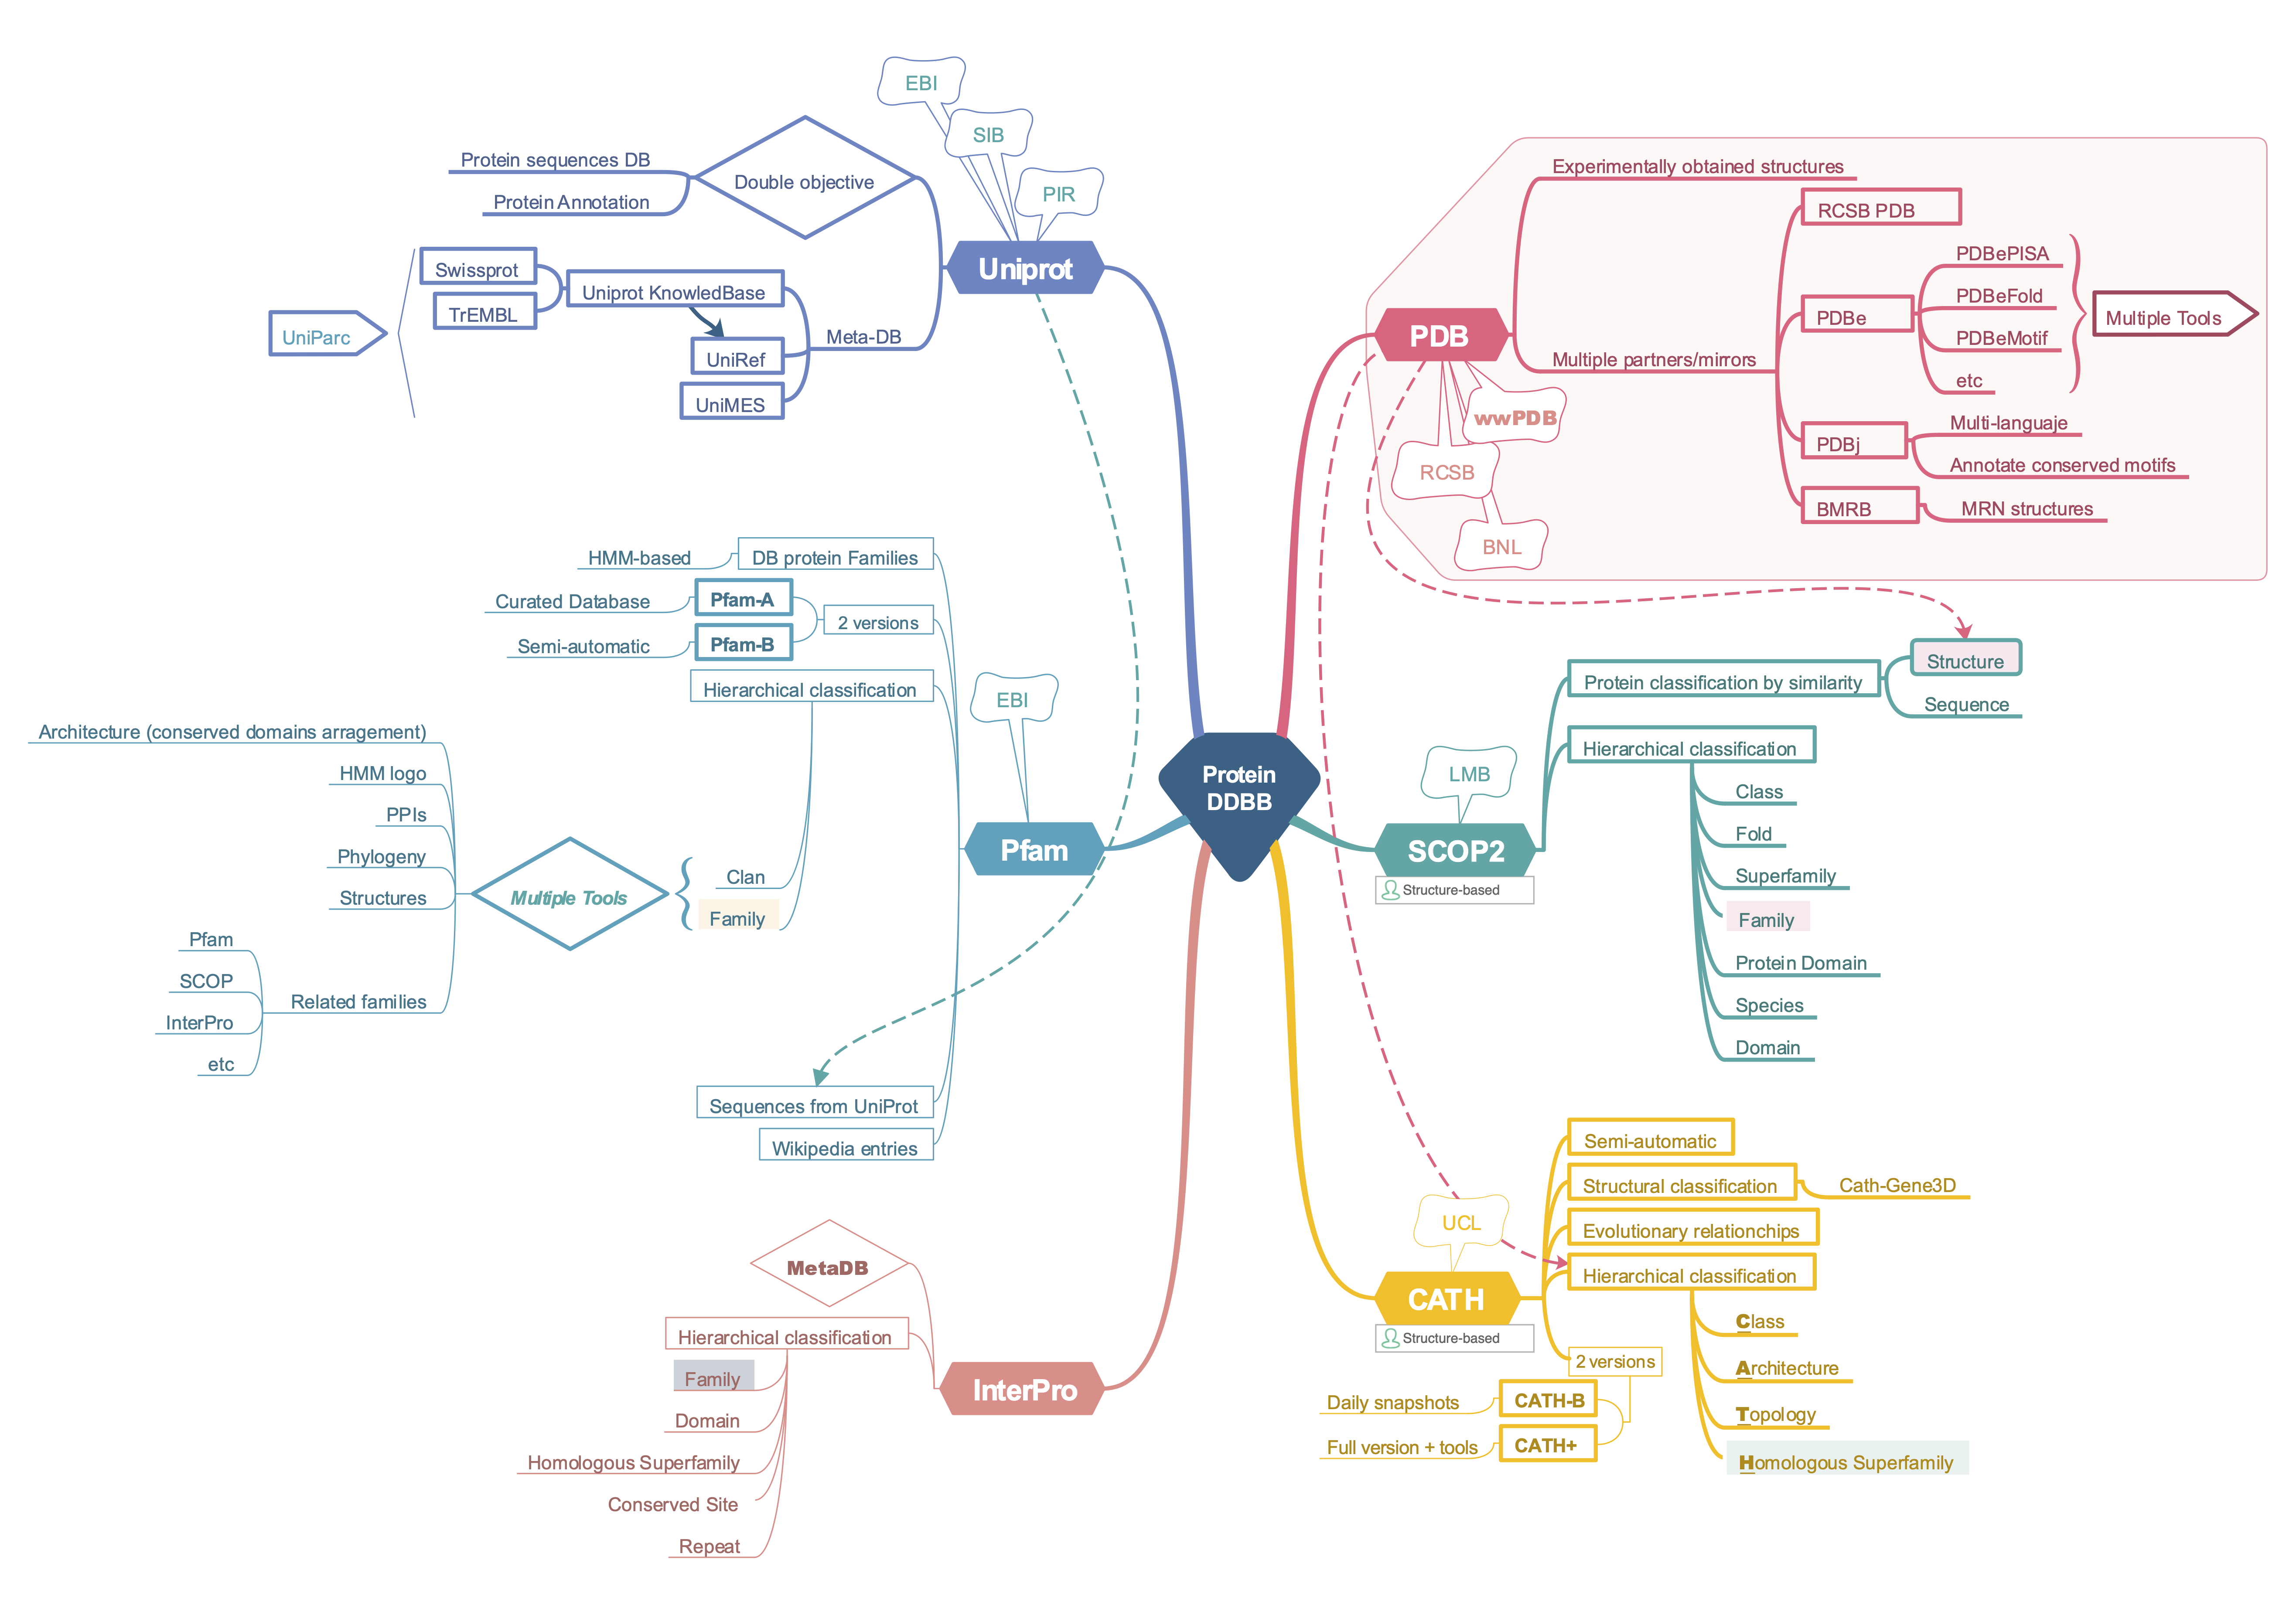
\includegraphics[width = 0.9\textwidth]{figs/bbdd_full.png}
\end{figure}

\begin{table}[htbp]
\begin{mdframed}[backgroundcolor=black!10]
    \centering
    Todas las bases de datos que describimos aquí permiten el acceso mediante programación y/o API, normalmente con paquetes BioPython y R, lo que aumenta significativamente las posibilidades de programación y análisis de datos por lotes.
    \end{mdframed}
\end{table}

\subsection{Bases de datos estructurales}
\subsubsection{RCSB-PDB}
La base de datos Protein Data Bank es la principal base de datos estructural primaria de macromoléculas. Contiene principalmente estructuras de proteínas, pero también abarca ácidos nucleicos y complejos nucleoproteicos. PDB cumplió 50 años en 2021 y se puede ver un resumen detallado de su historia en el sitio RCSB-PDB.

Brevemente, el PDB se creó en 1971 en el Laboratorio Nacional de Brookhaven con sólo 7 estructuras. Posteriormente, el \textbf{Research Collaboratory for Structural Bioinformatics (RCSB)}, formado por Rutgers, UCSD/SDSC y CARB/NIST, se hizo responsable de la gestión del PDB en 1998 en respuesta a una RFP y un largo proceso de revisión. En 2003, se creó el Worldwide Protein Data Bank (wwPDB) para mantener un único archivo PDB de datos estructurales macromoleculares a disposición libre y pública de la comunidad mundial. Está formado por organizaciones que actúan como centros de depósito, procesamiento y distribución de datos PDB.

Las estructuras del PDB se obtienen en gran medida mediante cristalografía de rayos X, pero acepta derivaciones de datos de EM y RMN desde 1989 y 1991, respectivamente. De hecho, el BMRB (Biological Magnetic Resonance Bank) se ha asociado con el PDB desde 2006 y el EMBD (Electron Microscopy Data Bank) desde 2021. Además, a partir de septiembre de 2022, el PDB también contiene modelos computados de la base de datos Alphafold (de la que hablaremos más adelante en este curso) y RoseTTAFold-ModelArchive. \textbf{Así pues, la base de datos PDB es el eje principal que centraliza las estructuras biológicas en la actualidad}.

La base de datos PDB tiene cuatro réplicas y sitios web (RCSB, Europa, BMRB y Japón) con información que se solapa principalmente, aunque tienen cierta especialización. El sitio PDB del RCSB tiene también una sección educativa (PDB-101) con información y recursos muy útiles para la enseñanza y el aprendizaje de la biología estructural y el trabajo con estructuras PDB.

%PREGUNTA EXAMEN: Verdadero o falso, PDB tiene estructuras computacionales

Las entradas del PDB contienen toda la información sobre la estructura, desde la secuencia de la proteína y su origen hasta los detalles del experimento, así como la evaluación de la estructura y la visualización. Se puede descargar toda esta información y las coordenadas de la estructura en diversos formatos de archivo.

\subsubsection{SCOP}
La base de datos Structural Classification of Proteins (SCOP, http://scop.mrc-lmb.cam.ac.uk) es una \textbf{clasificación de dominios proteicos} organizada según sus relaciones evolutivas y estructurales en categorías jerárquicas. La unidad principal es la \textbf{familia}, que agrupa proteínas relacionadas con pruebas claras de su origen evolutivo, mientras que la \textbf{superfamilia} reúne dominios proteicos relacionados de forma más distante. Además, las superfamilias se agrupan en \textbf{pliegues} distintos en función de las características estructurales globales que comparten la mayoría de sus miembros. Se proporcionan definiciones de dominio para los dos niveles principales de la clasificación SCOP, familia y superfamilia, y los límites de dominio para cada uno de ellos pueden coincidir o diferir.

Para cada grupo, se selecciona un representante basándose en su secuencia (UniProtKB) y estructura (PDB) y se utiliza para la clasificación SCOP. Así, los límites de dominio SCOP se asignan tanto a la entrada PDB como a la UniProtKB.

\subsubsection{CATH}
CATH (www.cathdb.info) es un recurso gratuito y de acceso público que identifica dominios proteicos dentro de proteínas del Banco de Datos de Proteínas y los clasifica en grupos relacionados evolutivamente según la información sobre secuencia, estructura y función. Parte de la base de que las proteínas relacionadas que se pliegan de forma similar suelen exhibir funciones similares (esto sólo podría demostrarse si encontramos intermediarios). CATH utiliza un esquema de clasificación jerárquica en el que las unidades comparadas y clasificadas son dominios estructurales. Los dominios, definidos aquí como dominios estructurales globulares capaces de plegarse de forma semiindependiente, se extraen de estructuras de proteínas determinadas experimentalmente y disponibles en la base de datos PDB. Los dominios se clasifican en los siguientes niveles jerárquicos que componen el nombre CATH: Clase (C), Arquitectura (A), Topología (T) y Superfamilias homólogas (H).

CATH utiliza una combinación de varios algoritmos basados en estructuras (SSAP, CATHEDRAL) y en secuencias (alineaciones de secuencias basadas en Needleman-Wunsch, Jackhmmer, Profile Comparer y HHsearch) para evaluar la similitud de los dominios entre sí e identificar proteínas homólogas.

CATH tiene un recurso hermano, Gene3D, que añade secuencias adicionales de dominios de proteínas sin estructura conocida, lo que eleva el número total actual de dominios en CATH-Gene3D a 95 millones.

La base de datos CATH se actualiza con bastante regularidad mediante instantáneas diarias (CATH-B), pero cada 12 meses se publica una versión completa con más herramientas, denominada CATH+. CATH-plus contiene familias funcionales (CATH-FunFams), clusters estructurales y otras herramientas.

\subsection{Bases de datos de secuencias}
\subsubsection{Uniprot}
Las bases de datos Uniprot están gestionadas por el consorcio UniProt, creado en 2002 por EMBL-EBI, SIB y PIR. En la actualidad, UniProt puede considerarse una metadatabase, ya que sus entradas contienen información procedente de diversas fuentes. Se creó con dos objetivos principales: establecer una base de datos de secuencias de proteínas completa y no redundante y enriquecer esa base de datos con anotaciones detalladas. Estas anotaciones incluyen familias de proteínas y genes, datos de función y estructura-función, interacciones con otras proteínas o cofactores, localización, patrones de expresión, variantes, etc. Así, pretende cumplir los objetivos tanto de las bases de datos primarias como de las secundarias.

El eje central de las bases de datos UniProt es la Uniprot Knowledgebase. Se trata de una colección de información funcional sobre proteínas, con anotaciones precisas, coherentes y ricas. UniProtKB consta de dos bases de datos internas: una sección contiene registros anotados manualmente con información extraída de la bibliografía, sugerencias de la comunidad y análisis computacionales revisados por los conservadores. La otra sección incluye registros analizados computacionalmente. Estas secciones se denominan «UniProtKB/Swiss-Prot» (revisada, anotada manualmente) y «UniProtKB/TrEMBL» (no revisada, anotada automáticamente), respectivamente.
En los últimos años, UniProtKB ha incorporado datos estructurales de la base de datos Alphafold, además de referencias cruzadas a información estructural. 

UniProt contiene secuencias con distintos niveles de detalle de anotación en dos bases de datos complementarias: Uniparc y Uniref. En resumen, UniParc (UniProt Archive) es una base de datos exhaustiva y no redundante que incluye la mayoría de las secuencias de proteínas disponibles públicamente en todo el mundo. UniParc evita la redundancia almacenando cada secuencia única una sola vez y asignándole un identificador único estable (UPI), que permite identificar la misma proteína a partir de diferentes bases de datos fuente. Un UPI nunca se elimina, cambia o reasigna. Por otro lado, UniRef (UniProt Reference Clusters) proporciona conjuntos agrupados de secuencias de UniProtKB (y registros seleccionados de UniParc) para garantizar una cobertura completa del espacio de secuencias a varias resoluciones, ocultando al mismo tiempo las secuencias redundantes (pero no sus descripciones). 
La base de datos UniRef100 combina secuencias idénticas en una única entrada UniRef, mostrando la secuencia de una proteína representativa, los números de acceso de todas las entradas fusionadas y enlaces a las bases de datos correspondientes. UniRef90 se construye agrupando secuencias UniRef100 utilizando el algoritmo MMseqs2, de modo que cada clúster consiste en secuencias con al menos un 90\% de identidad de secuencia y un 80\% de solapamiento con la secuencia más larga (la secuencia semilla ) del clúster. Del mismo modo, UniRef50 se construye agrupando secuencias semilla UniRef90 que tienen al menos un 50\% de identidad de secuencia y un 80\% de solapamiento con la secuencia más larga del clúster. UniParc y UniRef sólo contienen secuencias de proteínas; el resto de la información sobre las proteínas debe recuperarse de las bases de datos de origen utilizando referencias cruzadas de bases de datos.

\subsubsection{InterPro}
InterPro pretende ser una base de datos funcional secundaria, clasificando las proteínas en familias, dominios y sitios importantes. Para clasificar las proteínas de este modo, InterPro utiliza modelos predictivos, conocidos como firmas, proporcionados por varias bases de datos diferentes (hasta 13) que conforman el consorcio InterPro. InterPro combina esas diferentes firmas que representan familias, dominios o sitios equivalentes, y proporciona información adicional como descripciones, referencias bibliográficas y términos de la Ontología Genética (GO), para producir un recurso completo para la clasificación de proteínas.

La base de datos InterPro se actualiza cada 2 meses y es muy útil para la anotación de ORFans o proteínas divergentes. En los últimos años, ha integrado más recursos, incluyendo Pfam, así como datos estructurales y predicciones, dando lugar a un recurso muy práctico para múltiples propósitos en la ciencia de las proteínas.

Interpro se creó como una BBDD de secuencias, pero actualmente se encuentra en un punto intermedio. Ahora se podría decir que es más bien una «metabase de datos» que contiene información sobre secuencias y estructuras.

\subsubsection{Pfam}
Pfam es una base de datos de proteínas cuyo objetivo es clasificar secuencias por sus relaciones evolutivas. Se fundó en 1995 y ha sido muy útil para la anotación funcional de datos genómicos. El sitio web de Pfam (http://pfam.xfam.org/) se cerró a finales de 2022. Sin embargo, la base de datos Pfam no se interrumpió, sino que se integró en el sitio InterPro. Pfam utiliza perfiles HMM para clasificar las proteínas en familias, que se agrupan en clanes. 

La versión actual (37.1) contiene 23.794 entradas y 751 clanes. Pfam se diseñó como una base de datos que debe actualizarse con frecuencia en la era genómica de avance rápido. Para ello, utiliza dos tipos de alineación. Cada familia Pfam tiene un alineamiento semilla que contiene un conjunto representativo de secuencias para la entrada. A partir del alineamiento semilla se construye automáticamente un modelo de Markov oculto (HMM) de perfil y se busca en una base de datos de secuencias denominada pfamseq utilizando el software HMMER3 (http://hmmer.org/). Todas las regiones de secuencias que satisfacen un umbral curado específico de la familia, también conocido como umbral de reunión, se alinean con el HMM de perfil para crear el alineamiento completo.

Además de las entradas Pfam basadas en HMM (Pfam-A), los perfiles Pfam se utilizan para proporcionar un conjunto de alineaciones de secuencias múltiples no anotadas, generadas computacionalmente, denominadas Pfam-B. Sin embargo, en las últimas versiones de Pfam, los alineamientos Pfam-B sólo se publican actualmente en el sitio FTP de Pfam.

Pfam también se ha utilizado en la creación de otros recursos como Rfam (familias de ARN) y Dfam (elementos transponibles de ADN).

\section{Estrategias actuales y futuras en las bases de datos de proteínas}
Existe una tendencia significativa hacia el cruce y la integración de datos diversos dentro de las \textbf{metadatabases}. Un caso ejemplar es el Human Protein Atlas, que proporciona información sobre proteínas clasificadas por tipo celular o tejido, junto con detalles sobre variantes de splicing, mutantes, etc. Además, es importante reconocer las nuevas bases de datos estructurales, como la base de datos Alphafold de Deepmind y el Atlas Metagenómico ESM, que albergan millones de estructuras de proteínas predichas mediante métodos de aprendizaje profundo. También existen bases de datos especializadas, como BFDV, que contienen estructuras de proteínas víricas obtenidas a través de Alphafold (pero que no están en la base de datos de AlphaFold) y en las que se pueden realizar búsquedas mediante Foldseek, un método diseñado para identificar similitudes estructurales.

Dado el reciente impulso en la capacidad de obtener con precisión modelos de proteínas, algunos autores sugirieron (o desearon) que las futuras bases de datos contuvieran no solo variantes de secuencias de proteínas y complejos proteicos, sino también conformaciones diversas para cada estructura, lo que ayudaría a conocer mejor su función y papel biológico.



\end{document}
